\documentclass[a4paper]{scrartcl}
\usepackage{defaultstyle}
\usepackage{localstyle}

\title{Authorization Logic for App Policies}
\subtitle{Second Year Report}
\author{Joseph Hallett}
\date\today

\begin{document}
\maketitle

\begin{abstract}
  This report describes second year work of my PhD.
  I give a brief overview of the app installation policies and the AppPAL authorisation logic; before describing the work completed this year.
  I review what topics suggested in the thesis proposal.
  Work re-implementing AppPAL, exploring store and user policies and looking at protocols for app distribution is described.
  I describe what I expect to work on in the final year of my studies.
  Finally, I give a table of contents for the proposed thesis.
\end{abstract}

\section{Introduction}

Mobile devices let users pick the apps they want to run.
App stores offer a wide range of software for users to choose.
Users pick particular apps for a variety of reasons:
  ordering in the store~\citep{Prata:2012in},
  reviews and privacy concerns~\citep{Kelley:2013kc},
  and security rules from their employer.

Finding the right apps can be tricky:
  users need to work out which apps are well written, which are not going to abuse their data, which ones will work in the way they want
  and to find the apps which suit how they want to use their device.
This can be difficult as it isn't obvious how apps use the data each has access to.

People fall into patterns when thinking about the privacy issues around apps~\citep{Sadeh:2014vq}.
Companies have policies about how phones should be used by employees.
With \emph{bring your own device} schemes employees use their personal devices for work.
IT departments in these companies may need to create policies so that the devices can be used securely with company information.
Ensuring compliance is often left to the employees.

These policies exist for mobile ecosystems; but there aren't ways of modelling them precisely or enforcing them.
I believe that authorization logic can be used to describe these policies and enforce them automatically.
Authorization logic's can describe the trust relationships and policies surrounding Android formally.
This lets us to make precise statements about the security of these systems.
This can be used to make comparisons between different security models, such as those in iOS and Android.
It allows comparisons between user's privacy policy and their actual behaviour.

By capturing these patterns explicitly as policies they can be enforced automatically.
By checking the policies we can enforce them at run-time; or warn users when making decisions that go against their policies.
This reduces the burden on users to decide which apps they want.
Security-savvy users may design policies themselves: these could be shared with others or used in organisation-wide curated app stores.


This thesis research will show how authorization logic can be used to make security decisions in mobile devices.
Security decisions must be made manually by smart phone users
By automating these choices we believe users can avoid having to make security decisions and their overall security be improved.

\subsection{AppPAL}

AppPAL is an instantiation of SecPAL~\citep{Becker:2006vh} we have developed to model and enforce app installation policies.
Using AppPAL we can describe policies with trust relationships, and which incorporate constraints.
This gives us a powerful language which can be used to describe user's and companies app policies precisely.

AppPAL can express that a user finds they can install an AppPAL:
\begin{lstlisting}
`user' says `apk://com.rovio.angrybirds' isInstallable.
\end{lstlisting}
Or that an app is installable \emph{if} some conditions are correct and \emph{where} a constraint is true.
\begin{lstlisting}
`user' says App isInstallable
  if `office-app-policy' isMetBy(App)
  where locationAt(`work') = true.
\end{lstlisting}
Decisions can be delegated to other users; with separate versions where further delegation is allowed (\lstinline{inf}) or not (\lstinline{0}).
\begin{lstlisting}
`user' says `it-department' can-say 0 `office-app-policy' isMetBy(App).
\end{lstlisting}
And principals can be given roles or subjects renamed.
\begin{lstlisting}
`user' says `ian' can-act-as `it-department'.
\end{lstlisting}
Statements are collected into an \emph{assertion context} which is queried using SecPAL's three evaluation rules~\citep{Becker:2006vh}.


\section{Summary of second year work}

%\subsection{What I said I'd do}

I proposed primarily looking at the role of app stores this year in my thesis proposal.
Specifically I wanted to understand how users interacted with the stores.
This would enable us to better understand user behaviour.
By better understanding user behaviour I could write policies that accurately described the users.
I said that I would:
\begin{itemize}
  \item Implement an app store filtered by AppPAL policies.
  \item Look at how users interact with apps, and the kinds of policies they apply, as well as what happens when their policies change.
  \item Look at how the policies vary within categories of apps.
  \item Explore how policies could be composed and joined.
  \item Explore what happens when policies are attacked.
\end{itemize}

Several of these topics changed as year went on.
I implemented a system for creating app stores based on an AppPAL policy, but when I also gained access to real installation data.
Using this data I started to look at what apps users pick from stores and the kinds of policies they apply.
I started looking at greater detail at the distribution mechanisms and policies within app stores.

Some existing work continued on from the first year: AppPAL was reimplemented in Java to allow it to run on Android.
Other work was started from necessity.
I wanted a means of systematically running tools over large numbers of apps and collecting the results;
  so I built one and have used the data collected from it in other aspects of the project.

In the next few sections I describe work I have completed in the second year; and show findings.

\subsection{Re-implemented AppPAL in Java.}

In the first year we implemented a prototype AppPAL interpreter in Haskell.
Haskell lacks good ARM compilers, and cannot access Android libraries and APIs easily.
This made on device experimentation harder.
I re-implemented it in Java and made sure it was portable, running a library in an app, or Java program.
The current implementation contains roughly the same number of lines of code, but runs everywhere and is significantly easier to modify.

Performance of the library when searching an assertion context for proofs is reasonable.
The search procedure is at its slowest when performing large repeated delegations.
Two synthetic benchmarks were created to check that the search procedure performed acceptably.
Each benchmark consisted of repeated chain of delegations.
The \emph{straight} benchmark consists of a single long chain of delegation.
The \emph{forking} benchmark consists of a binary tree of principals delegating to each other.
These benchmarks are reasonable as they model the worst kinds of policies to evaluate---though worse ones could be designed by forking even more.

On a Nexus 4 device checking times are measured in seconds when there are hundreds of delegations in a single policy check, and in minutes when there are thousands (\autoref{fig:benchmarks}).
We have only used a few delegations per decision when describing hypothetical user policies.
Since the benchmarks show that long chains of delegation can be used, I believe the performance is acceptable.
AppPAL constraints will be the slowest part of checking a policy.
Since a constraint can execute arbitrary programs or include network requests their performance is independent of AppPAL.
In practice the only ones I have used (so far) are permissions checks.
These are very fast as they can call out to the Android package manager.
Slowly evaluating constraints could be used but this may lead to policy designed to limit the number of constraint checks.
Current practical policies check five or six permissions per app.
Since the numbers of checks are small it is not worth optimising (yet).

\begin{figure}
  \begin{minipage}{0.49\linewidth}
    \footnotesize
    \begin{tabular}{cccc}
       \toprule
       Policy   & Principals & Parse (s) & Check (s) \\
       \midrule
       Straight & 10    & 0.01      & 0.04      \\
       Straight & 100   & 0.05      & 1.00      \\
       Straight & 500   & 0.32      & 21.07     \\
       Straight & 1000  & 0.43      & 87.75     \\
       \midrule
       Forking  & 256   & 0.10      & 1.93      \\
       Forking  & 512   & 0.23      & 7.47      \\
       Forking  & 1024  & 0.45      & 28.29     \\
       Forking  & 2048  & 0.85      & 117.68    \\
       \bottomrule
    \end{tabular}
  \end{minipage}
  \begin{minipage}{0.49\linewidth}
    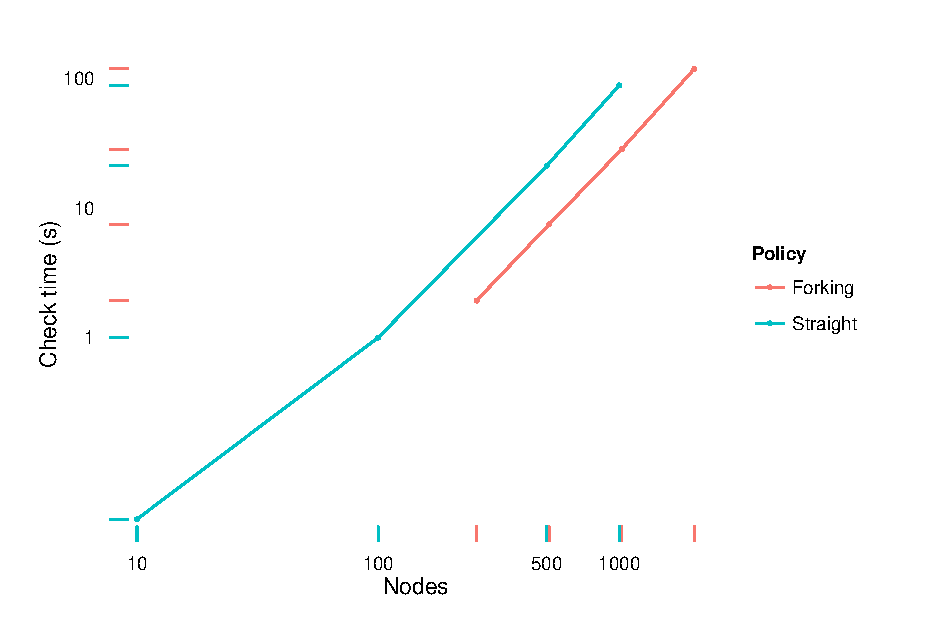
\includegraphics[width=\linewidth]{./images/benchmarks.eps}
  \end{minipage}
  \caption{Bench-marking results on a Nexus 4 Android phone.}
  \label{fig:benchmarks}
\end{figure}

\subsection{Built a \ac{SKB} exporting statements to AppPAL.}

As part of the AppPAL framework I imagined using results from static analysis tools as constraints within the language.
To collect and store these results I built an extensible \ac{SKB} that was lightweight and which could be trivially extended.
Implemented in Ruby the \ac{SKB} supports running metadata-fetching and static-analysis tools in parallel over large collection of apps.
Adding tools is quick and painless: add a library to Ruby, or a file to a configuration folder implementing a class interface---see \autoref{fig:fetcher}.

The \ac{SKB} exports statements to AppPAL, and holds around 40,000 apps at the moment.
Running the \texttt{skb dump} command causes the SKB to emit an AppPAL assertion context that can be used to make queries (\autoref{fig:dump}).
The \ac{SKB} can also emit statements from other principals where appropriate.
For example in \autoref{fig:dump} the \ac{SKB} emitted  statements from the Play store for the apps categorisation and review score.
Since the information was obtained from the Play store it makes sense to speak as it in this scenario.

Development of the \ac{SKB} is ongoing work.
One possible extension of the \ac{SKB} could be to store knowledge of vulnerabilities.
Hypothetically a device could warn a user if they attempt to install an app with a highly dangerous vulnerability.
\begin{lstlisting}
`user' says App requiresWarning
  if App hasCVSSScore(X)
  where X > 8.0.
\end{lstlisting}
The \ac{SKB} is designed to make fetching and storing these kinds of statement easy.
Its development will continue, as needed, into the next year.


\begin{figure}
  \centering
  \begin{Verbatim}[fontsize=\tiny]
$ skb dump
...
'skb' says `apk://com.olbg.tipsandroid' can-act-as `34458db1a8d0d1e0bca9bb658cf79872867d97b8' .
'PlayStore' says `34458db1a8d0d1e0bca9bb658cf79872867d97b8' hasReviewScore(`4.3').
'PlayStore' says `34458db1a8d0d1e0bca9bb658cf79872867d97b8' hasCategory(`Sports').
'skb' says `34458db1a8d0d1e0bca9bb658cf79872867d97b8' hasPermission(`android.permission.INTERNET').
'skb' says `34458db1a8d0d1e0bca9bb658cf79872867d97b8' hasPermission(`android.permission.ACCESS_NETWORK_STATE').
'skb' says `34458db1a8d0d1e0bca9bb658cf79872867d97b8' hasPermission(`android.permission.ACCESS_COARSE_LOCATION').
'skb' says `34458db1a8d0d1e0bca9bb658cf79872867d97b8' hasPermission(`android.permission.ACCESS_FINE_LOCATION').
'skb' says `34458db1a8d0d1e0bca9bb658cf79872867d97b8' hasPermission(`android.permission.WRITE_EXTERNAL_STORAGE').
'skb' says `34458db1a8d0d1e0bca9bb658cf79872867d97b8' hasPermission(`android.permission.READ_EXTERNAL_STORAGE').
'skb' says `34458db1a8d0d1e0bca9bb658cf79872867d97b8' hasCertificateVersion(`3 (0x2)').
'skb' says `34458db1a8d0d1e0bca9bb658cf79872867d97b8' hasCertificateSerial_Number(`2063699619 (0x7b018ea3)').
'skb' says `34458db1a8d0d1e0bca9bb658cf79872867d97b8' hasCertificateSignature_Algorithm(`sha256WithRSAEncryption').
'skb' says `34458db1a8d0d1e0bca9bb658cf79872867d97b8' hasCertificateIssuer(`O=Olbg').
'skb' says `34458db1a8d0d1e0bca9bb658cf79872867d97b8' hasCertificateNot_Before(`Aug 13 15:23:16 2013 GMT').
'skb' says `34458db1a8d0d1e0bca9bb658cf79872867d97b8' hasCertificateNot_After(`Aug  7 15:23:16 2038 GMT').
'skb' says `34458db1a8d0d1e0bca9bb658cf79872867d97b8' hasCertificateSubject(`O=Olbg').
'skb' says `34458db1a8d0d1e0bca9bb658cf79872867d97b8' hasCertificatePublic_Key_Algorithm(`rsaEncryption').
'skb' says `34458db1a8d0d1e0bca9bb658cf79872867d97b8' hasCertificatePublic-Key(`(2048 bit)').
'skb' says `34458db1a8d0d1e0bca9bb658cf79872867d97b8' hasCertificateExponent(`65537 (0x10001)').
'skb' says `34458db1a8d0d1e0bca9bb658cf79872867d97b8' hasCertificateX509v3_Subject_Key_Identifier(`').
'skb' says `34458db1a8d0d1e0bca9bb658cf79872867d97b8' hasCertificateSignature_Algorithm(`sha256WithRSAEncryption').
...
  \end{Verbatim}
  \caption{AppPAL output from the \ac{SKB}.}
  \label{fig:dump}
\end{figure}
\begin{figure}\centering
  \lstset{language=ruby,
          basicstyle  =\scriptsize\ttfamily,
          keywordstyle=\scriptsize\bfseries\ttfamily,
          stringstyle =\scriptsize\sffamily,
          commentstyle=\scriptsize\slshape\ttfamily}
  \begin{minipage}{0.48\linewidth}
    \begin{lstlisting}
require 'skb'

module ResultFetcher
  ##
  # Runs mallodroid on an APK
  class Mallodroid_HEAD < Skb::ResultFetcher
    ##
    # Timeout after 5 minutes
    def timeout
      300
    end

    def execute
      @out.puts `mallodroid
                  -x
                  -f "#{@apk.path}"`
      return true
    end
  end
end
    \end{lstlisting}
  \end{minipage}
  \begin{minipage}{0.48\linewidth}
    \begin{lstlisting}
require 'skb'
require 'zip/zip'

module MetaFetcher
  ##
  # Extracts the certificate used in the APK
  class Certificate < Skb::MetaFetcher
    def execute
      begin
        Zip::ZipFile.open @apk.path do |apk|
          cert = apk.find_entry \
            'META-INF/CERT.RSA'
          unless cert.nil?
            Dir.mktmpdir do |dir|
              cert.extract "#{dir}/CERT.RSA"
              out = `openssl pkcs7
                       -in '#{dir}/CERT.RSA'
                       -inform DERM
                       -print_certs |
                     openssl x509 -noout -text`
              @out << out
            end
            return true
          end
        end
        return false
      rescue => _e
        return false
      end
    end
  end
end
    \end{lstlisting}
  \end{minipage}
  \caption{Fetching plugins for Mallodroid and the certificate information for the \ac{SKB}.}
  \label{fig:fetcher}
\end{figure}

\subsection{Explored existing app store privacy policies.}

There are many Android app stores available.
I believed that each of the different stores would have different policies for kinds of apps, developers, and privacy conditions.
I read the privacy, developer and user policies for four different app stores (Google Play, Amazon, Aptoide and Yandex) to compare them.
In practice I found that the policies tended to be very similar; perhaps even copied in some places.
There were some differences when it came to payment processing, and minimum ages to use the store.
Some stores (excepting Google's) kept some right to modify any apps, typically for advertising.
This might form the basis of interesting trust relationships as the app would need to be re-signed by the store to be installed.
Re-signing is interesting because the trust in the authenticity of the app moves from the developer to the store.
A summary of the different terms and conditions is in \autoref{tab:terms}.

This work could be extended to help users pick an app store that is right for them, on the basis of policy.
Projects like COAT~\citep{Fernandez:5lFoplRA} aim to help users pick a store based on their privacy requirements.
We could imagine a similar scheme where AppPAL is used to help developers decide which stores to submit their apps to,
  and which stores users should buy from.
For example a developer may only agree to sell their app on a store if the store lets them set their own price and they get a 75\% cut of the profits.
\begin{lstlisting}
`dev' says `selling-policy' isMetBy(Store)
  if `dev' setsPriceIn(Store),
     Cut isCutIn(Store).
  where Cut > 0.75.
\end{lstlisting}.
\autoref{tab:terms} could be translated into AppPAL to decide which stores can sell the apps; and on the basis of this policy only Aptoide would be acceptable.

In Europe and America the choice of which market to use is not interesting as only Google's (and to an extent Amazon's) has enough market share to be compelling, and is pre-installed on most devices.
In China, however, where the Play store is banned by the government, there is a greater choice of marketplace and this becomes a more compelling avenue of research.

\begin{figure}[!h]\tiny
\begin{tabulary}{\linewidth}{lLLLL}
\toprule
                     & Google Play
                     & Amazon
                     & Yandex
                     & Aptoide \\ \midrule
User ID              & Name address and billing details.
                     & Amazon ID.
                     & None for free apps, payment details for paid.
                     & Contact details. No verification but agreement not to lie.                                                                                                        \\ \addlinespace
Client info taken    & Installation data, device ID, browsing history, cookies. Can opt out.
                     & Device ID, network info, location, usage data.
                     & Device ID, SIM number, Device content, System data, browsing history.
                     & Transaction history.  They may share it with developers.                                                                                                          \\ \addlinespace
Customer Payments    & Google Wallet and others at Google's discretion.
                     & Amazon.
                     & Approved processor by Yandex or store operator.
                     & Approved processor by Aptoide.                                                                                                                                    \\ \addlinespace
Who is paid?         & Google Commerce.
                     & Amazon.
                     & Developer.
                     & Store owner.                                                                                                                                                      \\ \addlinespace
Prices set by        & Developer.
                     & Amazon.
                     & Developer (but Yandex may restrict to set values).
                     & Developer and store owner.                                                                                                                                        \\ \addlinespace
Refunds              & Only for defective or removed content. A refund may be requested for two hours after purchase.
                     & No.
                     & Up to 15 minutes after purchase. No for IAP.
                     & Up to 24 hours after purchase.                                                                                                                                     \\ \addlinespace
Age of use           & At least 13.
                     & Any age (with consent of guardian).  No alcohol related content bellow 21.
                     & At least 14.
                     & A legal age to form a contract with Aptoide.                                                                                                                      \\ \addlinespace
Update provision     & You agree to receive updates.
                     & By default.
                     & Yes for security and bug-fixes.
                     & Yes agree to receive updates.                                                                                                                                     \\ \addlinespace
Moderation           & No obligation (but they may).
                     & Publisher obliged to provide info which may be used to give ratings.  Amazon will not check these ratings are accurate.
                     & No obligation (but they may).
                     & No obligation (but they may).  Trusted app mark does not indicate moderation.                                                                                     \\ \addlinespace
Acceptable use       & No use as part of a public performance, or for dangerous activities where failure may lead to death.
                     &
                     &
                     & No modification, rental, distribution or derivative works.  You may use the software.                                                                             \\ \addlinespace
Store rights to app  & Marketing and optimising Android.
                     & Distribution, evaluation, modification, advertising, and creating derivatives for promotion.
                     & Advertising.
                     & Modification and re-selling.                                                                                                                                      \\ \addlinespace
Withdrawal from sale & Immediate.
                     & 10 days, or 5 days if for copy-write reasons.
                     & 90 days. A copy will be retained.
                     & You may.                                                                                                                                                          \\ \addlinespace
Developer ID         & Google account and billing details.
                     & Amazon ID.
                     & Email, company name, tax-id.
                     & Email (preferably a Google developer one).                                                                                                                        \\ \addlinespace
EULA                 & Default offered.
                     & Only if it doesn't interfere with Amazon's terms.
                     & Must be provided.
                     & Default offered                                                                                                                                                   \\ \addlinespace
Content restrictions & No alternate stores, sexual, violence, IP infringing, PII publishing, illegal, gambling, malware, self-modifying or system modifying content.  No unpredictable network use.
                     & No offensive, pornography, illegal, IP infringing or gambling content.
                     & No defects. No illegal, disruptive, sexual, IP infringing, PII stealing, alternative stores, or open-source content.
                     & No displaying or linking to illegal, privacy interfering, violent, PII stealing, IP infringing content.  Nothing \emph{spammy} or with unpredictable network use. \\ \addlinespace
Payout rates         & 70\% of user's payment.
                     & 70\% list price (minus card fees).
                     & 70\% net-revenue (minus card fees).
                     & 75\% revenue share (minus card fees).                                                                                                                             \\ \addlinespace
\bottomrule
\end{tabulary}
\caption{Summary of conditions in different stores.}
\label{tab:terms}
\end{figure}

\subsection{Explored distribution mechanisms in existing stores.}

A user buying an app probably wants the app sent to their device.
Using an SSL proxy I started looking at the precise distribution mechanisms and started reverse engineering their protocols.
For simple website stores, such as Opera's mobile store, where apps are distributed without encryption it is trivial to modify downloaded apps on the fly.
A \ac{MITM} attack using a tool like can \texttt{mitmproxy} can modify the apps as they are downloaded.
In these stores there was no verification that the app downloaded matched the app requested.

Various security issues were found in other stores.
Amazon's store was the only one to enable certificate pinning.
The only pinned certificate was for accessing the login server.
Once the user had logged on, an SSL proxy could be used to examine traffic.
This meant that the store prevented you from logging on to the store when traffic was modified in a \ac{MITM} attack.
Once the login token had been issued, however the traffic between the store and the device could be intercepted and decrypted freely.
This isn't in itself bad as certificate pinning is not often required (though it probably should be in this scenario) but is interesting.

Google's store occasionally seemed to drop encryption when downloading APK files.
To download an app from the store the user has to follow a protocol, which we describe in abstract terms in \autoref{fig:protocol}.
This was inferred by looking at the network traffic and reverse-engineering the store APK file.
After completing the purchase the user presents their proof-of-purchase token to the store along with a description of the app their identifier (messages 5 \& 6)
The store tells then tells them a server to speak to which provides the app to them without further information (the blank message 7 and message 8).
This is implemented in practice using a URL redirect, where $S$ and $S^\prime$ are servers.
What we observed, however, is that occasionally the redirect was to a server using HTTP rather than HTTPS.
This meant that an attacker sniffing the traffic could see which apps were being downloaded and take a copy for themselves.
If the sniffing party was an employer and usage of the app gave away personal information (say a diabetes app or Grindr) then could be problematic.
By replaying message seven the user (or a third-party who sniffed the URL) could re-download the app for up to a week later.

I would like to continue this work into the next year.
Each of the stores I looked at had a slightly different protocol for buying apps and a different means of downloading them onto the device.
I might imagine in an AppPAL-enhanced app store apps being supplied with some assertions about their behaviour.
Working out how to include these in the download protocols, (and with knowledge distribution in general, proposed in \autoref{ssec:kdp}) seems interesting.

\begin{figure}[!h]
  \begin{minipage}{0.48\linewidth}
    \begin{center}
    \begin{tabular}{rrc}
      \toprule
      1. & $C \longrightarrow S$:        & $U, C, a_{\text{d}} $  \\ \addlinespace
      2. & $S \longrightarrow C$:        & $a_{\text{d}}, ? $     \\ \addlinespace
      3. & $C \longrightarrow S$:        & $U, ! $                \\ \addlinespace
      4. & $S \longrightarrow C$:        & $a_{\text{d}}, \$ $    \\ \addlinespace
      5. & $C \longrightarrow S$:        & $U, a_{\text{d}}, \$ $ \\ \addlinespace
      6. & $S \longrightarrow C$:        & $S^\prime$             \\ \addlinespace
      7. & $C \longrightarrow S^\prime$: &                        \\ \addlinespace
      8. & $S^\prime \longrightarrow C$: & $a$                    \\
      \bottomrule
    \end{tabular}
  \end{center}

    {\footnotesize In message 6, $S$ redirects $C$ using a 302-redirect message.
      By replaying message 7 I found I could re-download the app on a different client.
      I found that the redirection to the other server sometimes did not use SSL.}
  \end{minipage}
  \begin{minipage}{0.48\linewidth}
    \begin{tabulary}{\linewidth}{cC}
      \toprule
      Symbol         & Meaning                                                           \\
      \midrule
      $S$            & Store (\texttt{android.clients.google.com}).                      \\
      $C$            & Client the app store app running on the phone.                    \\
      $U$            & User, identified by a token.                                      \\
      $a$            & An app.                                                           \\
      $a_{\text{d}}$ & a description of the app $a$.                                     \\
      $?$            & Purchase challenge                                                \\
      $!$            & Purchase challenge response (seemingly derived from $?$ and $U$). \\
      $\$$           & Download token.                                                   \\
      $S^\prime$     & Alternate store URL                                               \\
      \bottomrule
    \end{tabulary}
  \end{minipage}
  \caption{Abstraction of the protocol used by Google's Play store to purchase an app.}
  \label{fig:protocol}
\end{figure}

\subsection{User app installation behaviour}

Mobile device users have policies about what data apps should be able to collected.
Lin~\etal~\citep{Sadeh:2014vq} identified four different privacy policies when users think about apps; however they did not look at whether they enforced them in practice.
Using AppPAL I implemented a simplification of the policies Lin~\etal~identified.
The Carat project~\citep{Oliner:2013ht} collected app installation data from users who installed their energy tracking app.
They shared this data with us in an anonymised form where I could see who had installed what provided I knew the package names of the apps they installed.
Ignoring system apps, using the \ac{SKB} I de-anonymised 4,300 apps (5\%) which accounted for 50\% of all app installs.
I selected 44,000 users for whom I knew 20 or more app installs.

Using the Carat data I measured the extent each user conformed with the privacy policies.
I also took a list of known malware and \acp{PUP} from McAfee to measure the extent of malware installations on Android.
From this I tested whether users who enforce their privacy policies install less malware.

I found that very few users follow these policies all the time.
A few users, however, do seem to be installing apps meeting a policies most of the time (\autoref{sfig:lin}).
For the unconcerned policy (the most permissive) only 1,606 users (4\%) had 50\% compliance;
and only 120 users (0.3\%) had 80\% compliance.
For the stricter conservative policy only 60 users were complying half the time, and just 7 more than 80\% of the time.
This suggests that while users may have privacy preferences the majority are not attempting to enforce them.

I found 1\% of the users had a PUP or malicious app installed (\autoref{sfig:malware}).
A user is three times more likely to have a PUP installed than malware.
Only nine users had both a PUP and malware installed.
Users who were complying more than half the time with the conservative or advanced policies complied with the malware or PUP policies fully (\autoref{sfig:compare}).
This is significant (P-value $< 0.05$) and suggests that users who pick their apps carefully are less likely to experience malware.

\begin{figure}\centering
  \begin{subfigure}[b]{0.48\linewidth}
    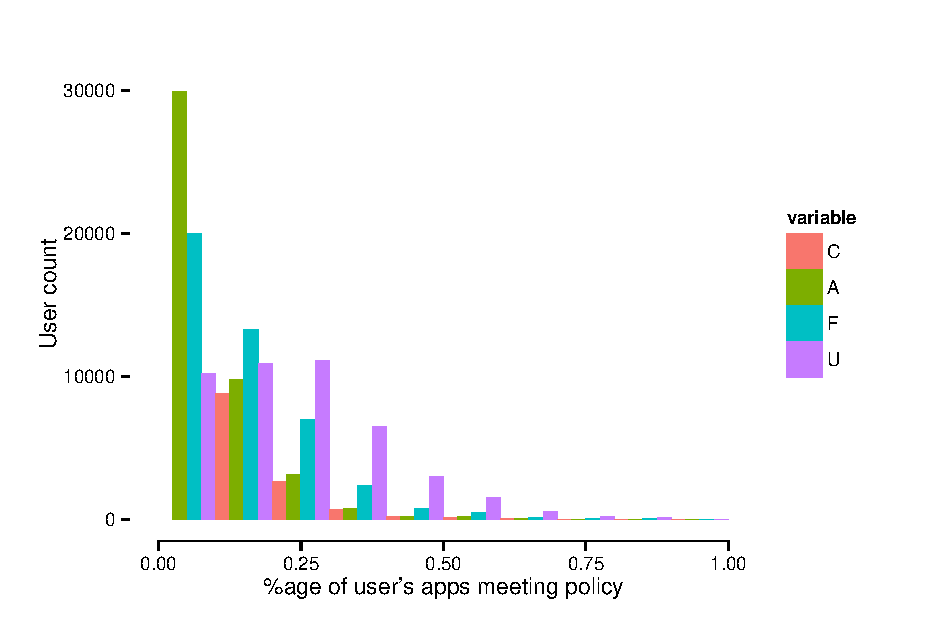
\includegraphics[width=\linewidth]{./images/lin-2yr.eps}
    \caption{User conformance to identified privacy policies.}
    \label{sfig:lin}
  \end{subfigure}
  \begin{subfigure}[b]{0.48\linewidth}
    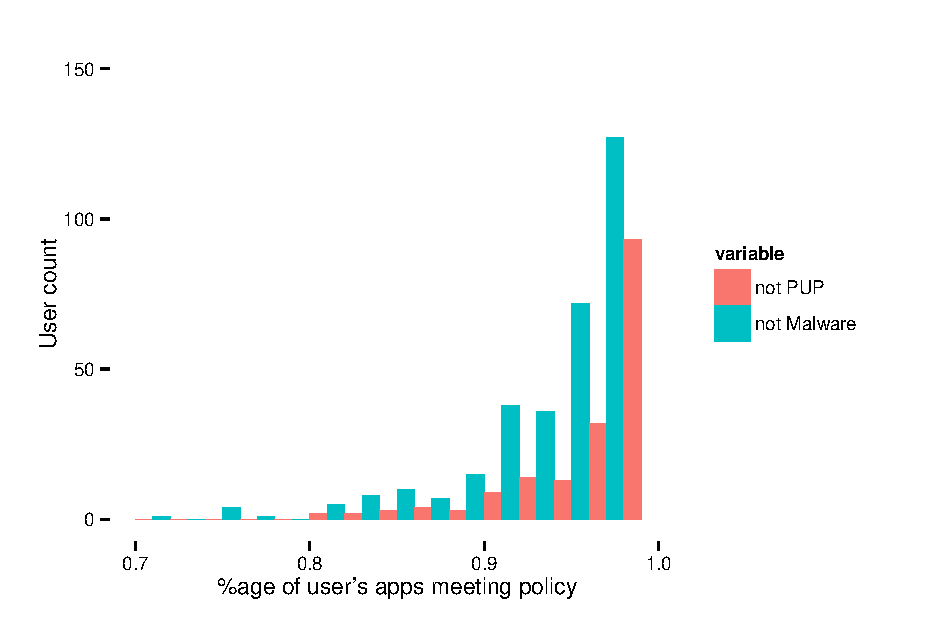
\includegraphics[width=\linewidth]{./images/malware-2yr.eps}
    \caption{User malware installation rates.}
    \label{sfig:malware}
  \end{subfigure}

  \begin{subfigure}[b]{\linewidth}
    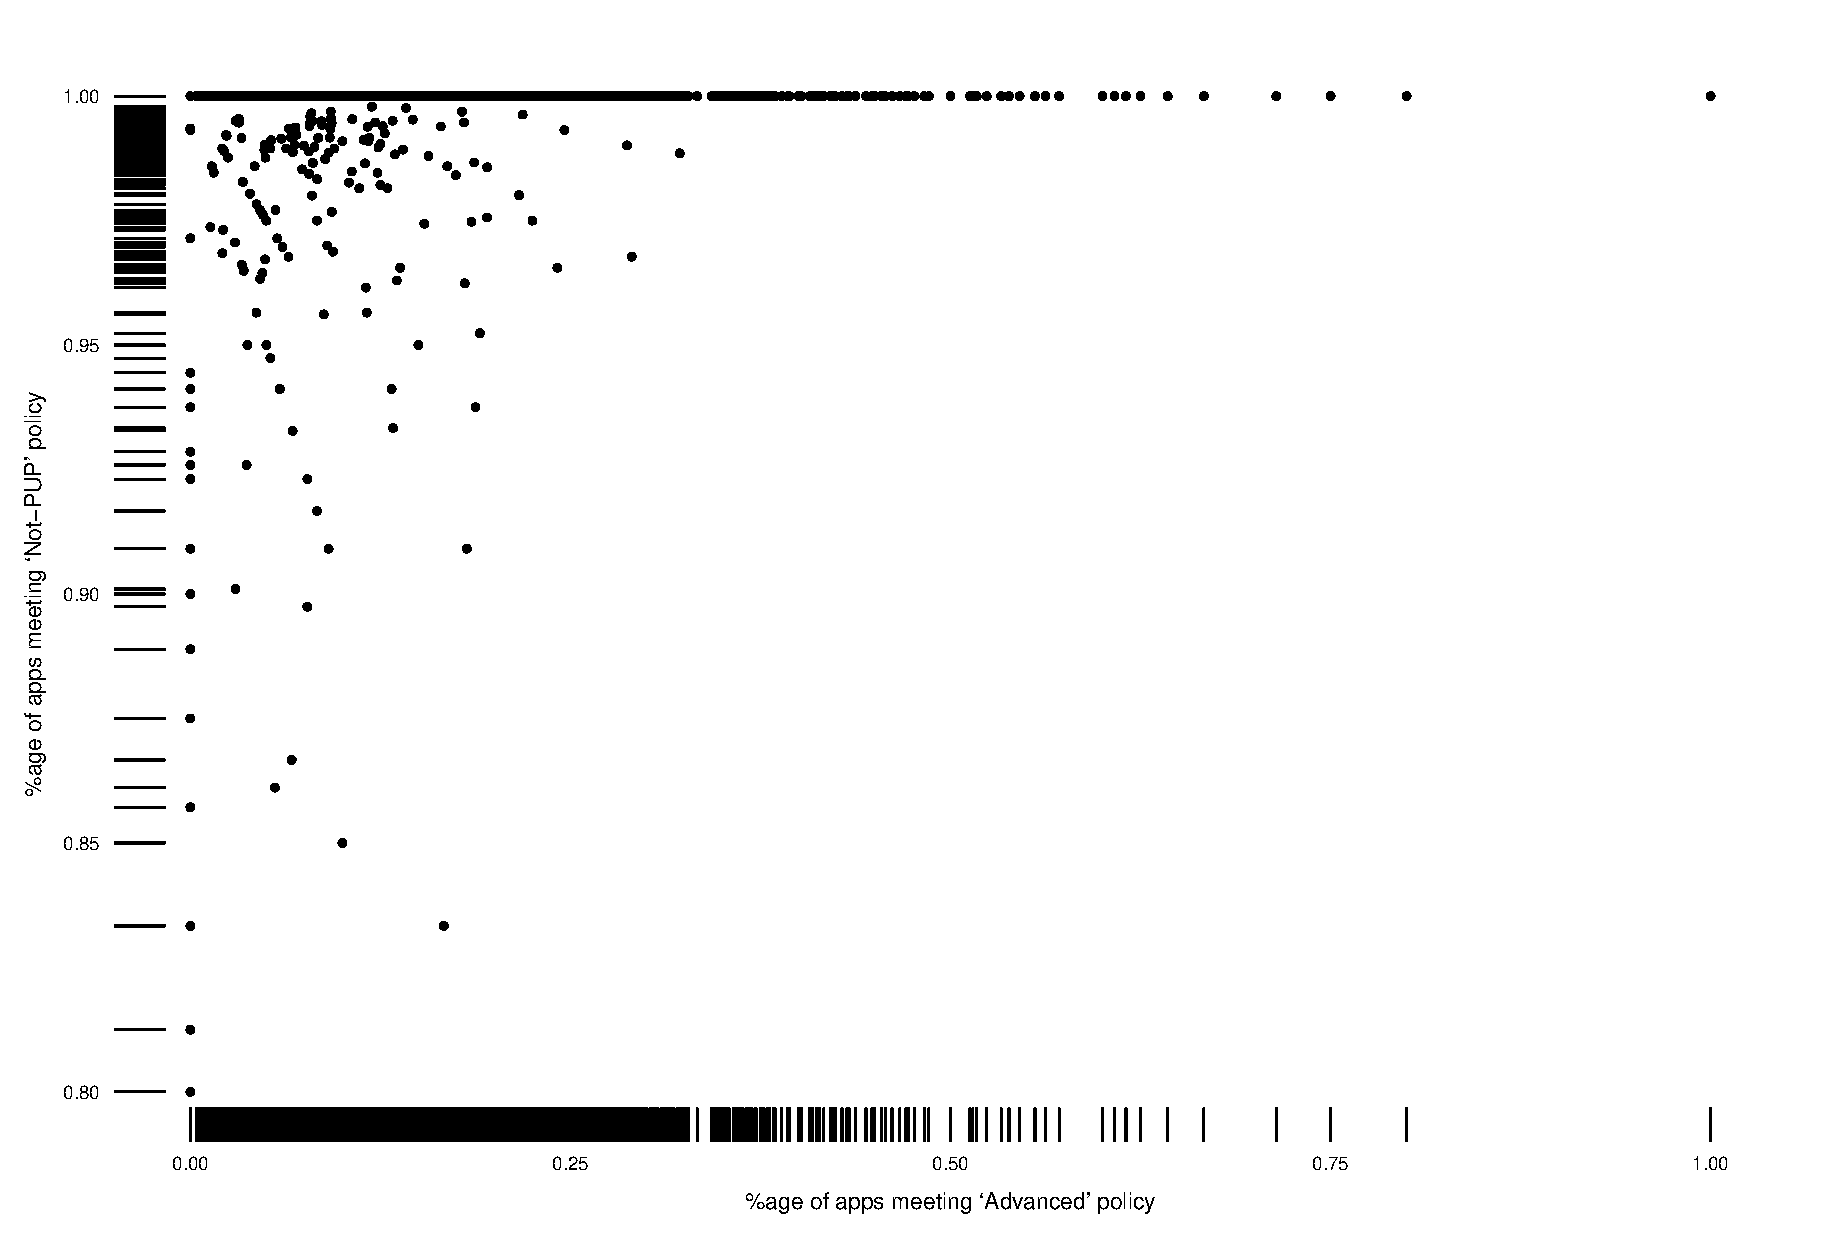
\includegraphics[width=\linewidth]{./images/compare-2yr.eps}
    \caption{Comparison of users following the advanced policy with malware installation.}
    \label{sfig:compare}
  \end{subfigure}

  \caption{Results from study on user app installation behaviour.}
  \label{fig:lin}
\end{figure}

This work was presented as a poster at SOUPS~\citep{Hallett:2015ty}, and I are aiming to publish it fully as part of a paper targeting the ESSoS conference (a draft of which is attached in an appendix).

\section{Next directions}

In the thesis proposal I suggested that in the third year I might look at advanced kinds of policies.
I also wanted to look at what might happen when policies have to deal with updates, to policies and apps on the device.
Some included:
\begin{itemize}
  \item The app collusion problem.
  \item What happens when policies are composed?
  \item Policy revocation and modification.
  \item App update policies.
\end{itemize}

Some of these problems have become less interesting: for example app updates.
Various different policies for updates could be encoded in AppPAL for the precise behaviour of an update.
Since most stores mandate accepting updates in the user agreement and the default behaviour is to auto-install updates schemes are unrealistic.
Updates typically include bug-fixes so it is in the user's interests to accept them (despite what they may believe~\citep{Vaniea:2014fk}).
Implementing methods to weaken security does not seem to be worthwhile.
Using AppPAL as a modelling language to precisely describe the trust mechanisms and delegations in an update is interesting.
It might make sense to include a comparison of the different update mechanisms in the thesis.

Policy modification is less interesting.
Apps should be rechecked before they can be allowed to run again.
If they now break the policy, the user should be prompted to remove the app or make an exception.
Results from long-running static analysis tools can be stored by the \ac{SKB}.
These could be reused by AppPALs constraint mechanisms to avoid re-computation, if no other changes were made.

The app collusion problem is interesting.
Whilst it is conceivable that AppPAL policies could describe and prevent attacks, to actually implement the protection in a way that could be used would probably require modifications to the intent system, and potentially binder (Android's primary IPC mechanism) and this probably makes it out of scope of the PhD.

The mechanisms for mechanically composing policies in AppPAL are trivial\footnote{\lstinline{`user' says `composed-policy' isMetBy(App)  if `pol1' isMetBy(App), `pol2' isMetBy(App).}} but what might happen when two principals actively disagree is more interesting.
AppPAL doesn't have support for negation, but it feels right that there should be some way to distinguish between a principal saying an app meets, does not meet, or does not know whether it meets a policy.
Continuing research should continue along with the protocols for distributing AppPAL statements.

\subsection{Knowledge distribution protocol}
\label{ssec:kdp}

AppPAL can enforce policies and I have started looking at the kinds of policies users might want to use.
When describing AppPAL policies I have thought about delegation relationships and how different principals can be trusted to help make decisions.
What isn't necessarily clear is how these principals get to make these statements and how they are transferred from speaker to speaker.

On a memory constrained device, like a mobile phone, storing a database of all possible ground AppPAL statements by every speaker is not viable.
There are almost 1.5 million apps available on the Google Play store, not including other stores or multiple versions of the same app.
Storing data on all apps will not work.
In the papers on SecPAL~\citep{Becker:2006vh,Becker:2009vt} (on which AppPAL is based) there is little talk about how the knowledge should be distributed.
They describe how principals should sign their AppPAL statements to identify themselves as having said them, and how an X.509-style public key system could be used to tie keys to principals.  This tells us how to check the statements are not forged but doesn't give the distribution mechanisms.
Related languages~\citep{Becker:2009ula,Aziz:2011vt,Gurevich:2008fz,Gurevich:Qo5E3M3} extended SecPAL language features but also didn't specify the distribution protocol.
SecPAL was built to be a distributed language with principals delegating statements.
Without a distribution protocols some scenarios can become difficult.

Consider Alice who wants to install an app on her phone.
Her installation policy requires confirmation the app is not malware.
She knows that McAfee can say (possibly with further delegation) whether an app is malicious or not;
  but this is a new app and she does not have any prior information about it.
She needs to get more information.
This scenario raises more questions:

\begin{itemize}
  \item How does she ask McAfee about the app?  What is the protocol for speaking and distributing statements?
  \item If the app is new McAfee may not know about it either. How should she send it to them for analysis?  What should she do while she waits: keep waiting, fail and keep a note to recheck later or fail and never ask again about the app?  Are there legal issues surrounding Alice redistributing the app to McAfee?
  \item How do McAfee respond?  AppPAL does not contain negation but in this scenario it would be helpful to distinguish a statement from McAfee that the app is safe, from one where they know it is definitely malware, from one where they are unsure and wish to err on the side of caution and not make a definite statement.
  \item If McAfee wish to delegate the decision they could issue another \emph{can-say} statement.   Should McAfee send the public key and any statements from the delegated party to the user, or just the server address and a reference to the public key on a PKI server?
  \item When should Alice ask McAfee?  Before any evaluation would be the easiest time as it would require no change to the evaluation algorithm but during the evaluation might be more appropriate as statements could be imported as needed.
\end{itemize}

Work this year should look at developing a strategy, and defining a protocol to share and acquire knowledge through AppPAL statements on demand.
This would be a worthwhile contribution, as it is novel, and would help extend AppPAL from a SecPAL instantiation to its own language.


\subsection{Case study}

Having an authorization logic model and enforce a real world policy shows the limitations and expressivity of a language.
It also shows that it is applicable to current compliance problems and solves \emph{real world problems} rather than just the policies I have learnt from user behaviour.

A natural source of these real world policies is corporate \ac{BYOD} policies, where employers describe restrictions on the usage of mobile devices in the workplace.
The \ac{NIST} have published recommendations for mobile device security and \ac{BYOD} in the workplace~\citep{Souppaya:2013jf,Scarfone:2009vy}.
Translating the mobile device relevant sections into AppPAL and showing their enforcement might make a good case study.
The study would focus on any difficulties in translating the policies and the extent the policy could be enforced automatically.

AppPAL policies I have used so far have been synthetic.
This has been fine for testing and demonstrating the language, but a larger example drawn from a real policy would help give AppPAL credibility.


\section{Proposed thesis outline}

\begin{quote}
  \emph{Hypothesis.} Automatic tools and policy languages would provide a
  better means of enforcement for mobile device policies than existing
  mechanisms which rely on manual inspection.
\end{quote}

\begin{enumerate}
  \item Introduction
  \item Mobile ecosystems
    \begin{description}
      \item[App stores and mobile app deployment]
        \hfill
        \begin{itemize}
          \item Introduce app stores and current development practices.
          \item Show the differences between different market places and the platforms (iOS vs Android).
        \end{itemize}
      \item[Android Security Model]
        \hfill
        \begin{itemize}
          \item Introduce the android permissions model and how different apps can access functionality provided by the platform.
          \item Show how app signing works.
        \end{itemize}
      \item[Android policies]
        \hfill
        \begin{itemize}
          \item Introduce the need for policies and the motivation for the PhD.
          \item Show how users do not seem to be following their privacy policies.
          \item Explain how some companies have mobile device policies, and how users are frustrated with data leaks.
          \item Show existing tools, such as Kirin, and explain why they're not good enough.
        \end{itemize}
    \end{description}
  \item AppPAL Implementation
    \begin{description}
      \item[The need for a policy language]
        \hfill
        \begin{itemize}
          \item Introduce scenarios where AppPAL can be used to enforce a policy
          \item Show trust relationships between different principals (a user at work).
          \item Start to introduce the language.
        \end{itemize}
      \item[Design and implementation of AppPAL]
        \hfill
        \begin{itemize}
          \item Formally present the language, as an instantiation of SecPAL.
          \item Show evaluation algorithm.
        \end{itemize}
    \end{description}
  \item AppPAL Experimentation
    \begin{description}
      \item[Deployment]
        \hfill
        \begin{itemize}
          \item Show applications using AppPAL.
          \item Stores generated by policy.
          \item On device policy checking.
          \item Device configuration by policy (if I can get access to Android M features)
        \end{itemize}
      \item[Distribution]
        \hfill
        \begin{itemize}
          \item Define protocol for knowledge acquisition.
          \item Describe implementation of protocol.
        \end{itemize}
    \end{description}
  \item Evaluation
    \begin{description}
      \item[User privacy policies]
        \hfill
        \begin{itemize}
          \item Show privacy paradox with Android apps.
          \item Use Carat (and McAfee?) data as a model of what users have installed.
          \item Shows power of AppPAL as a query and modelling language.
        \end{itemize}
      \item[Case study]
        \hfill
        \begin{itemize}
          \item Show how I can take a corporate policy and enforce it using AppPAL.
          \item Show the language is expressive enough to describe real policy scenarios.
          \item Shows that AppPAL can describe corporate policies that someone might want to use rather than synthetic examples.
        \end{itemize}
    \end{description}
  \item Related work
  \item Future work
\end{enumerate}

\bibliography{report}

\newpage
\appendix

\section{Paper for ESSoS 2016}

The attached paper is a draft being prepared for the ESSoS\footnote{Engineering Secure Software and Systems} symposium.
The paper will introduce the AppPAL language and its implementation.
I give sanity checking benchmarks to show its performance is not unreasonable.
Finally, I demonstrate AppPAL by presenting our work using AppPAL to filter user's privacy policies from our SOUPS poster, as part of a full paper.

\newgeometry{left=0.01em,top=0.01em, right=0.01em, bottom=0.01em}
\includepdf[pages=-]{../essos-2016-apppal/paper.pdf}

\end{document}

